% !TEX encoding = UTF-8 Unicode
%!TEX root = ../Main/thesis.tex
% !TEX spellcheck = en-US
%%=========================================
\documentclass[../Main/thesis.tex]{subfiles}
\begin{document}
\chapter{Third Iteration - Second prototype}
\label{ch:development-2}
This chapter describes the third, and final, iteration of the development process.
In this iteration the prototypes from Chapter~\ref{ch:development-1} improved and tested.

\section{Android application}
The Android application went through some changes in this iteration.
The most visible change is a new design for the app.
Some of the design changes are shown in Figure~\ref{fig:new-design}.
It was redesigned to be more user friendly and consistent with the design of the exercise management tool.

\begin{figure}[h]
	\centering
	\begin{subfigure}{0.2\textwidth}
		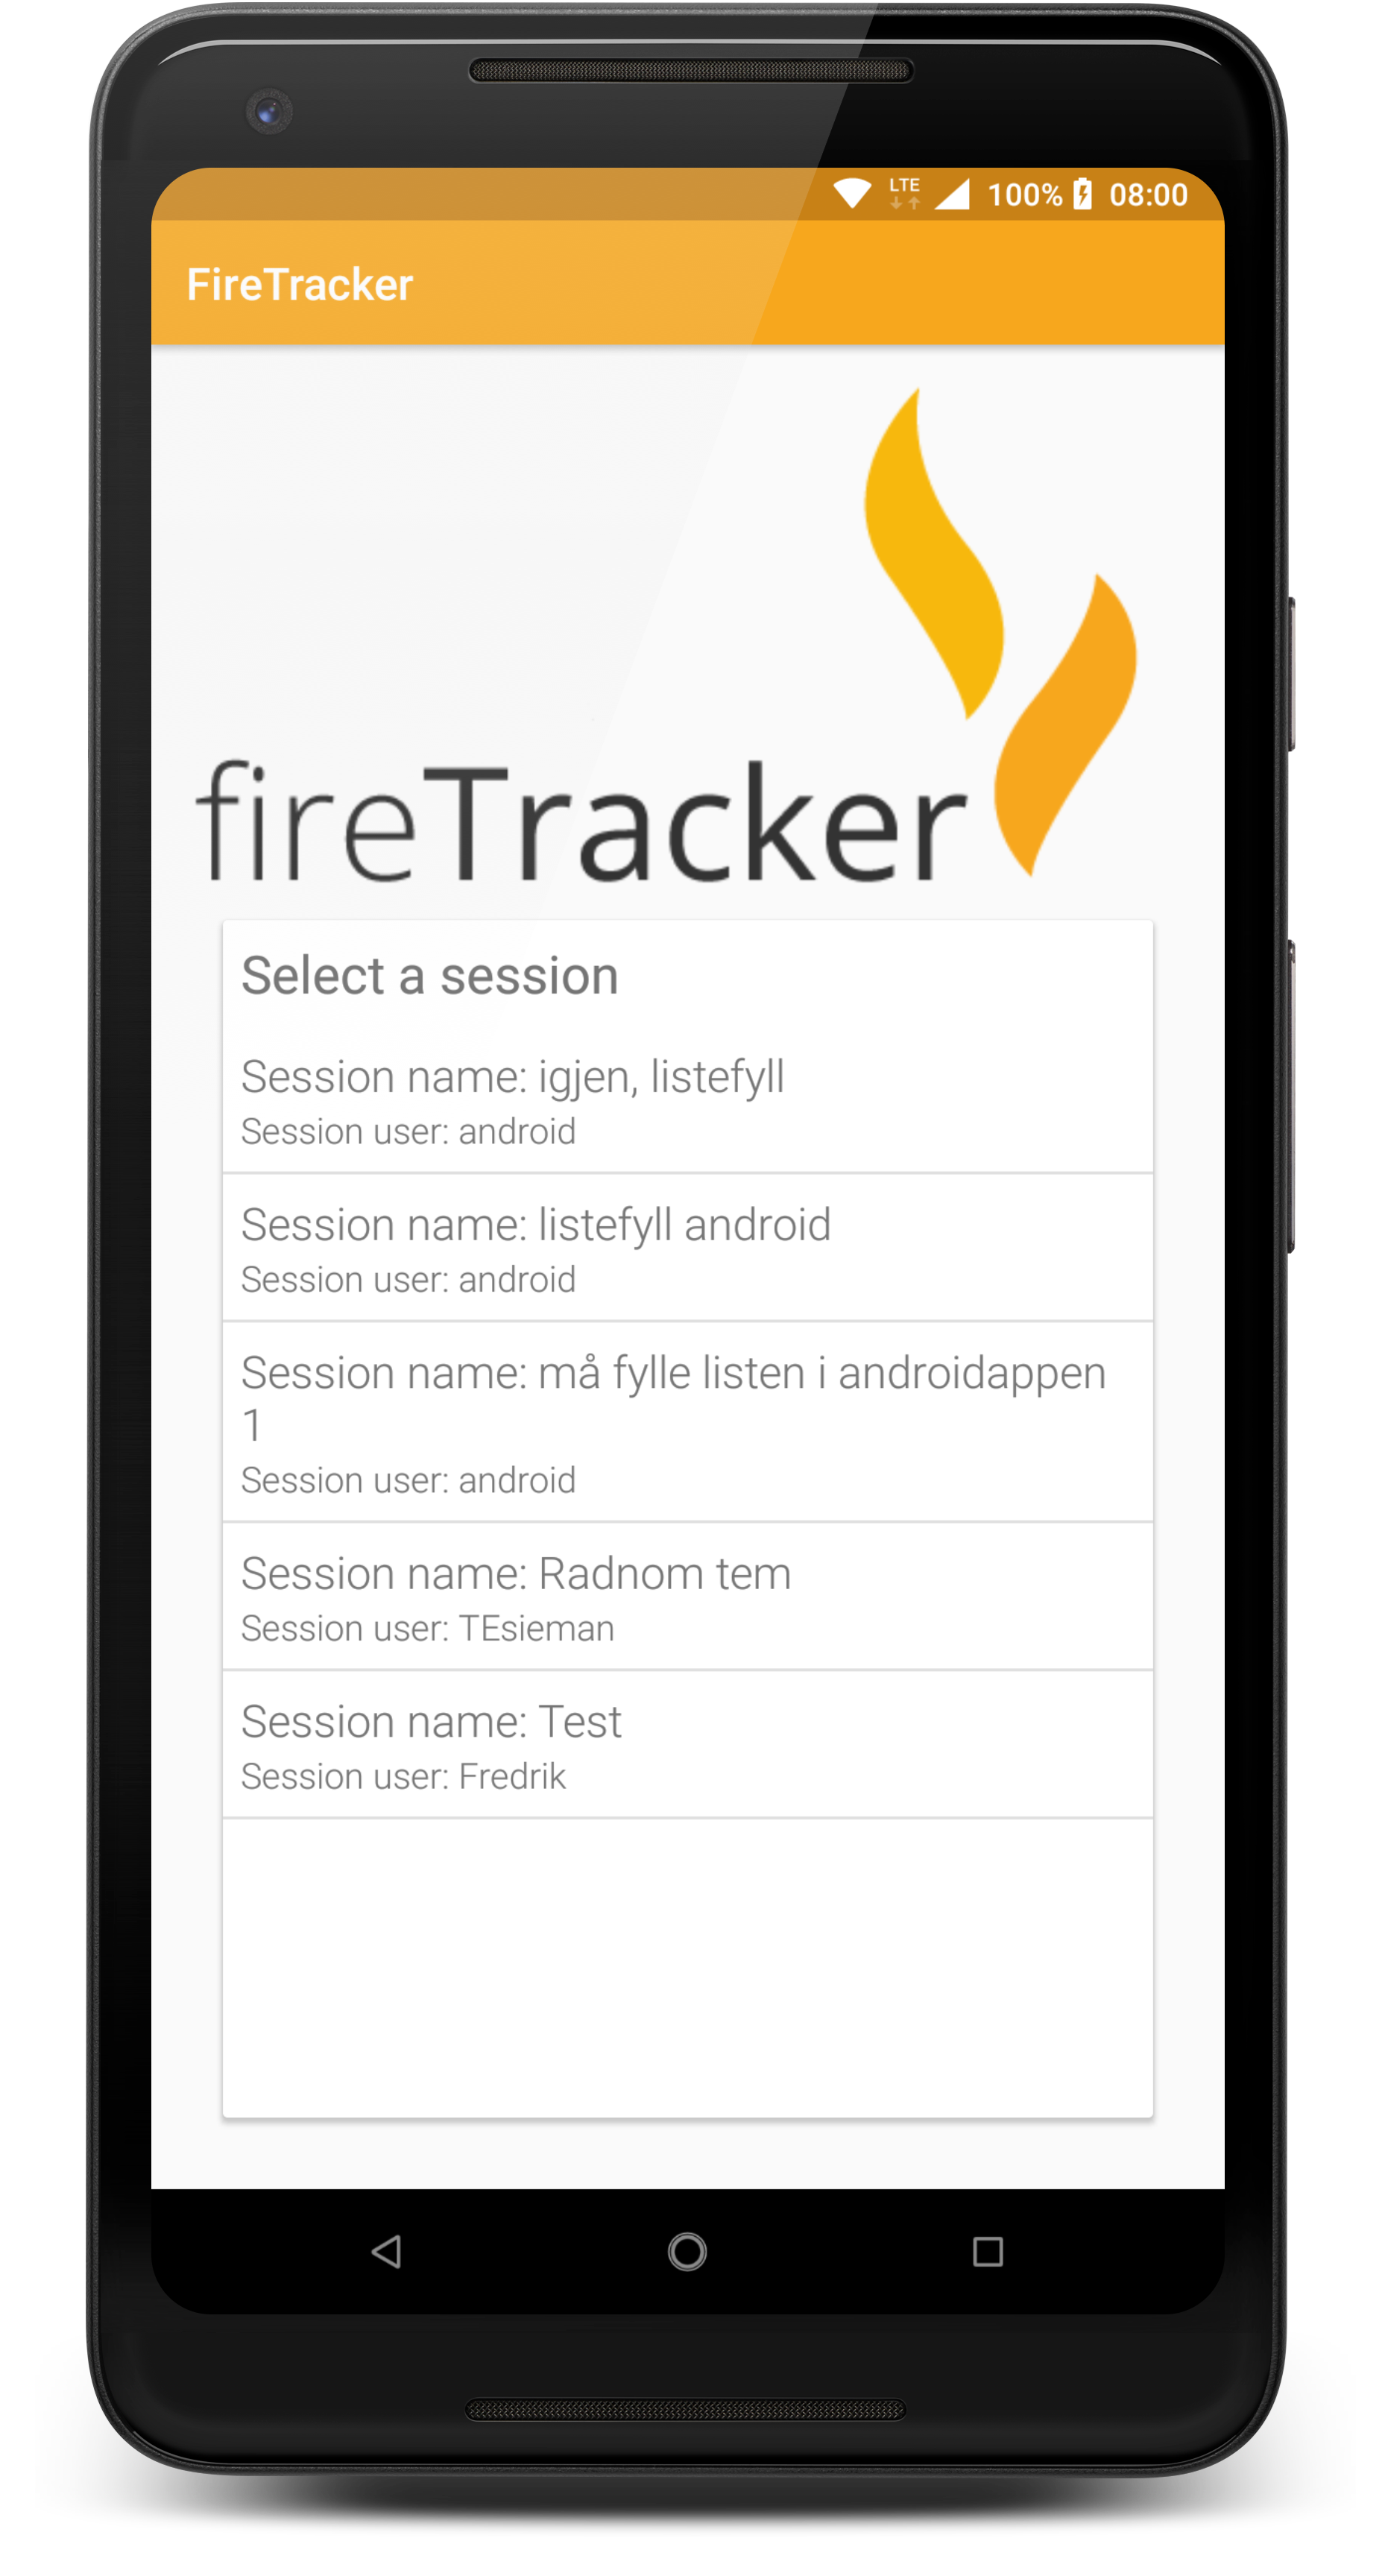
\includegraphics[width=\textwidth]{../fig/firetracker_app_old_1}
		\caption{Old design}
		\label{fig:app-old-design-sessionlist-iteration3}
	\end{subfigure}
	\begin{subfigure}{0.2\textwidth}
		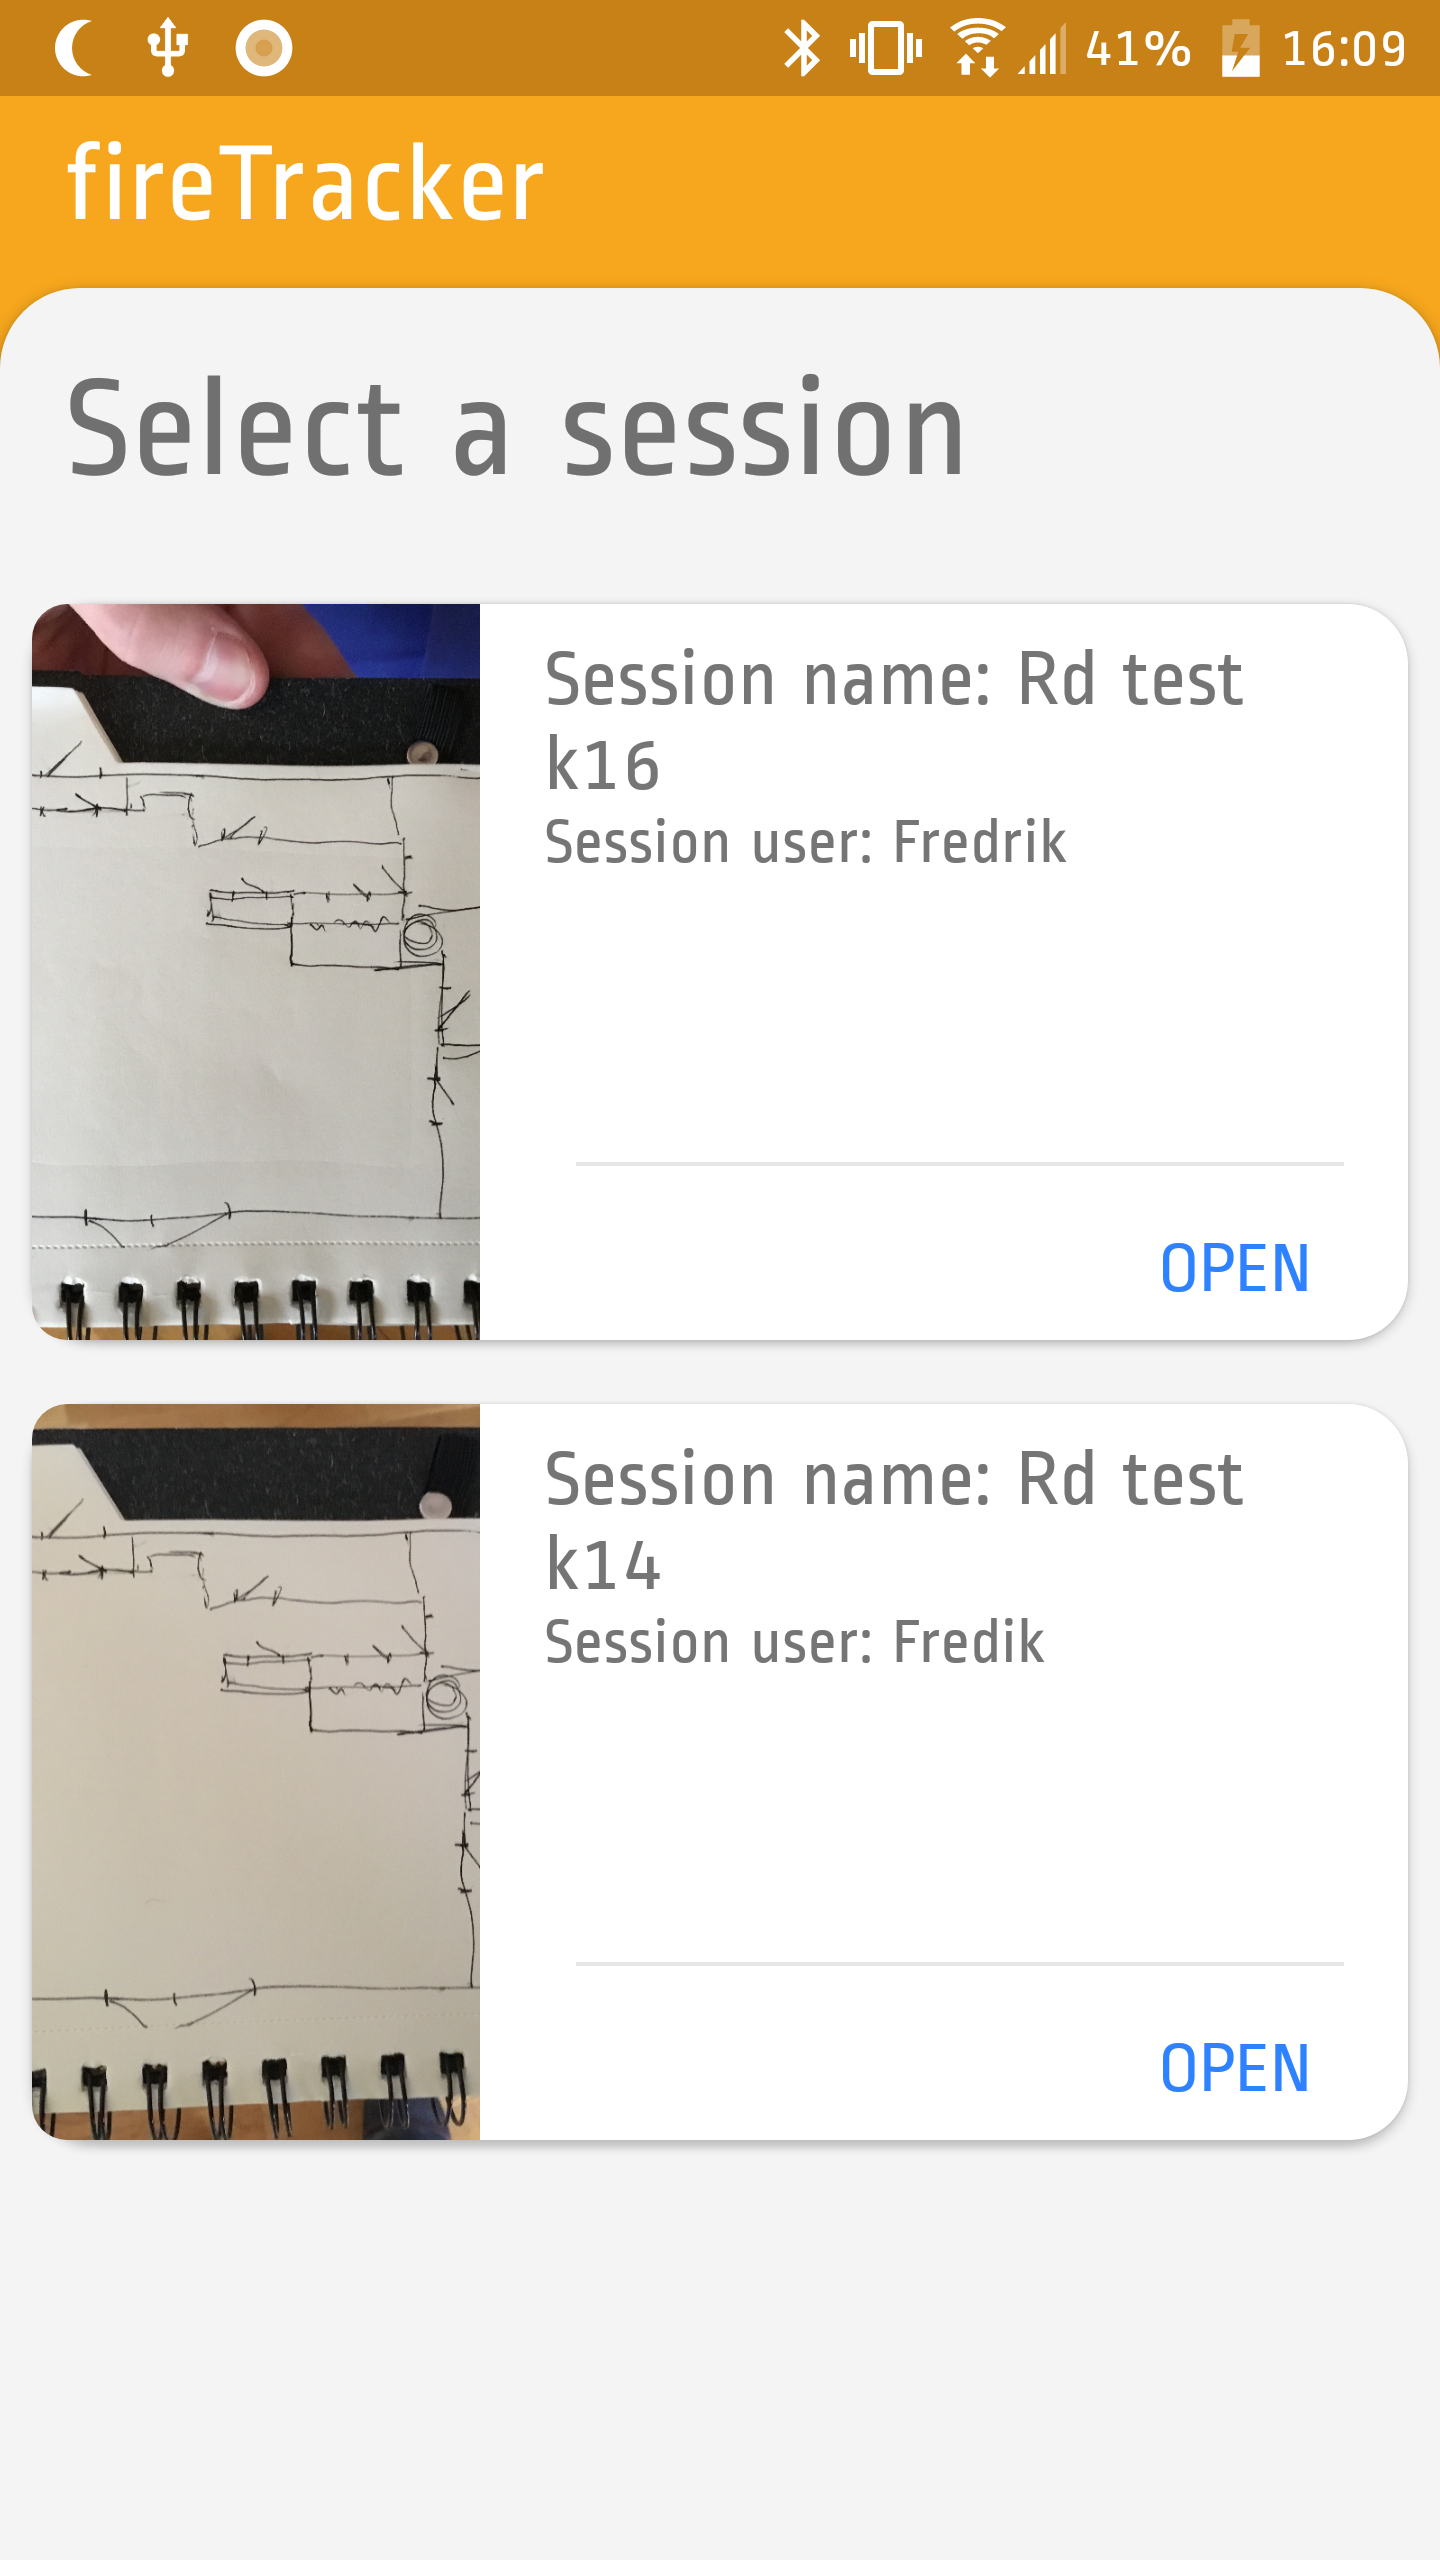
\includegraphics[width=\textwidth]{../fig/firetracker_app_new_1}
		\caption{New design}
		\label{fig:app-new-design-sessionlist-iteration3}
	\end{subfigure}
	\begin{subfigure}{0.2\textwidth}
		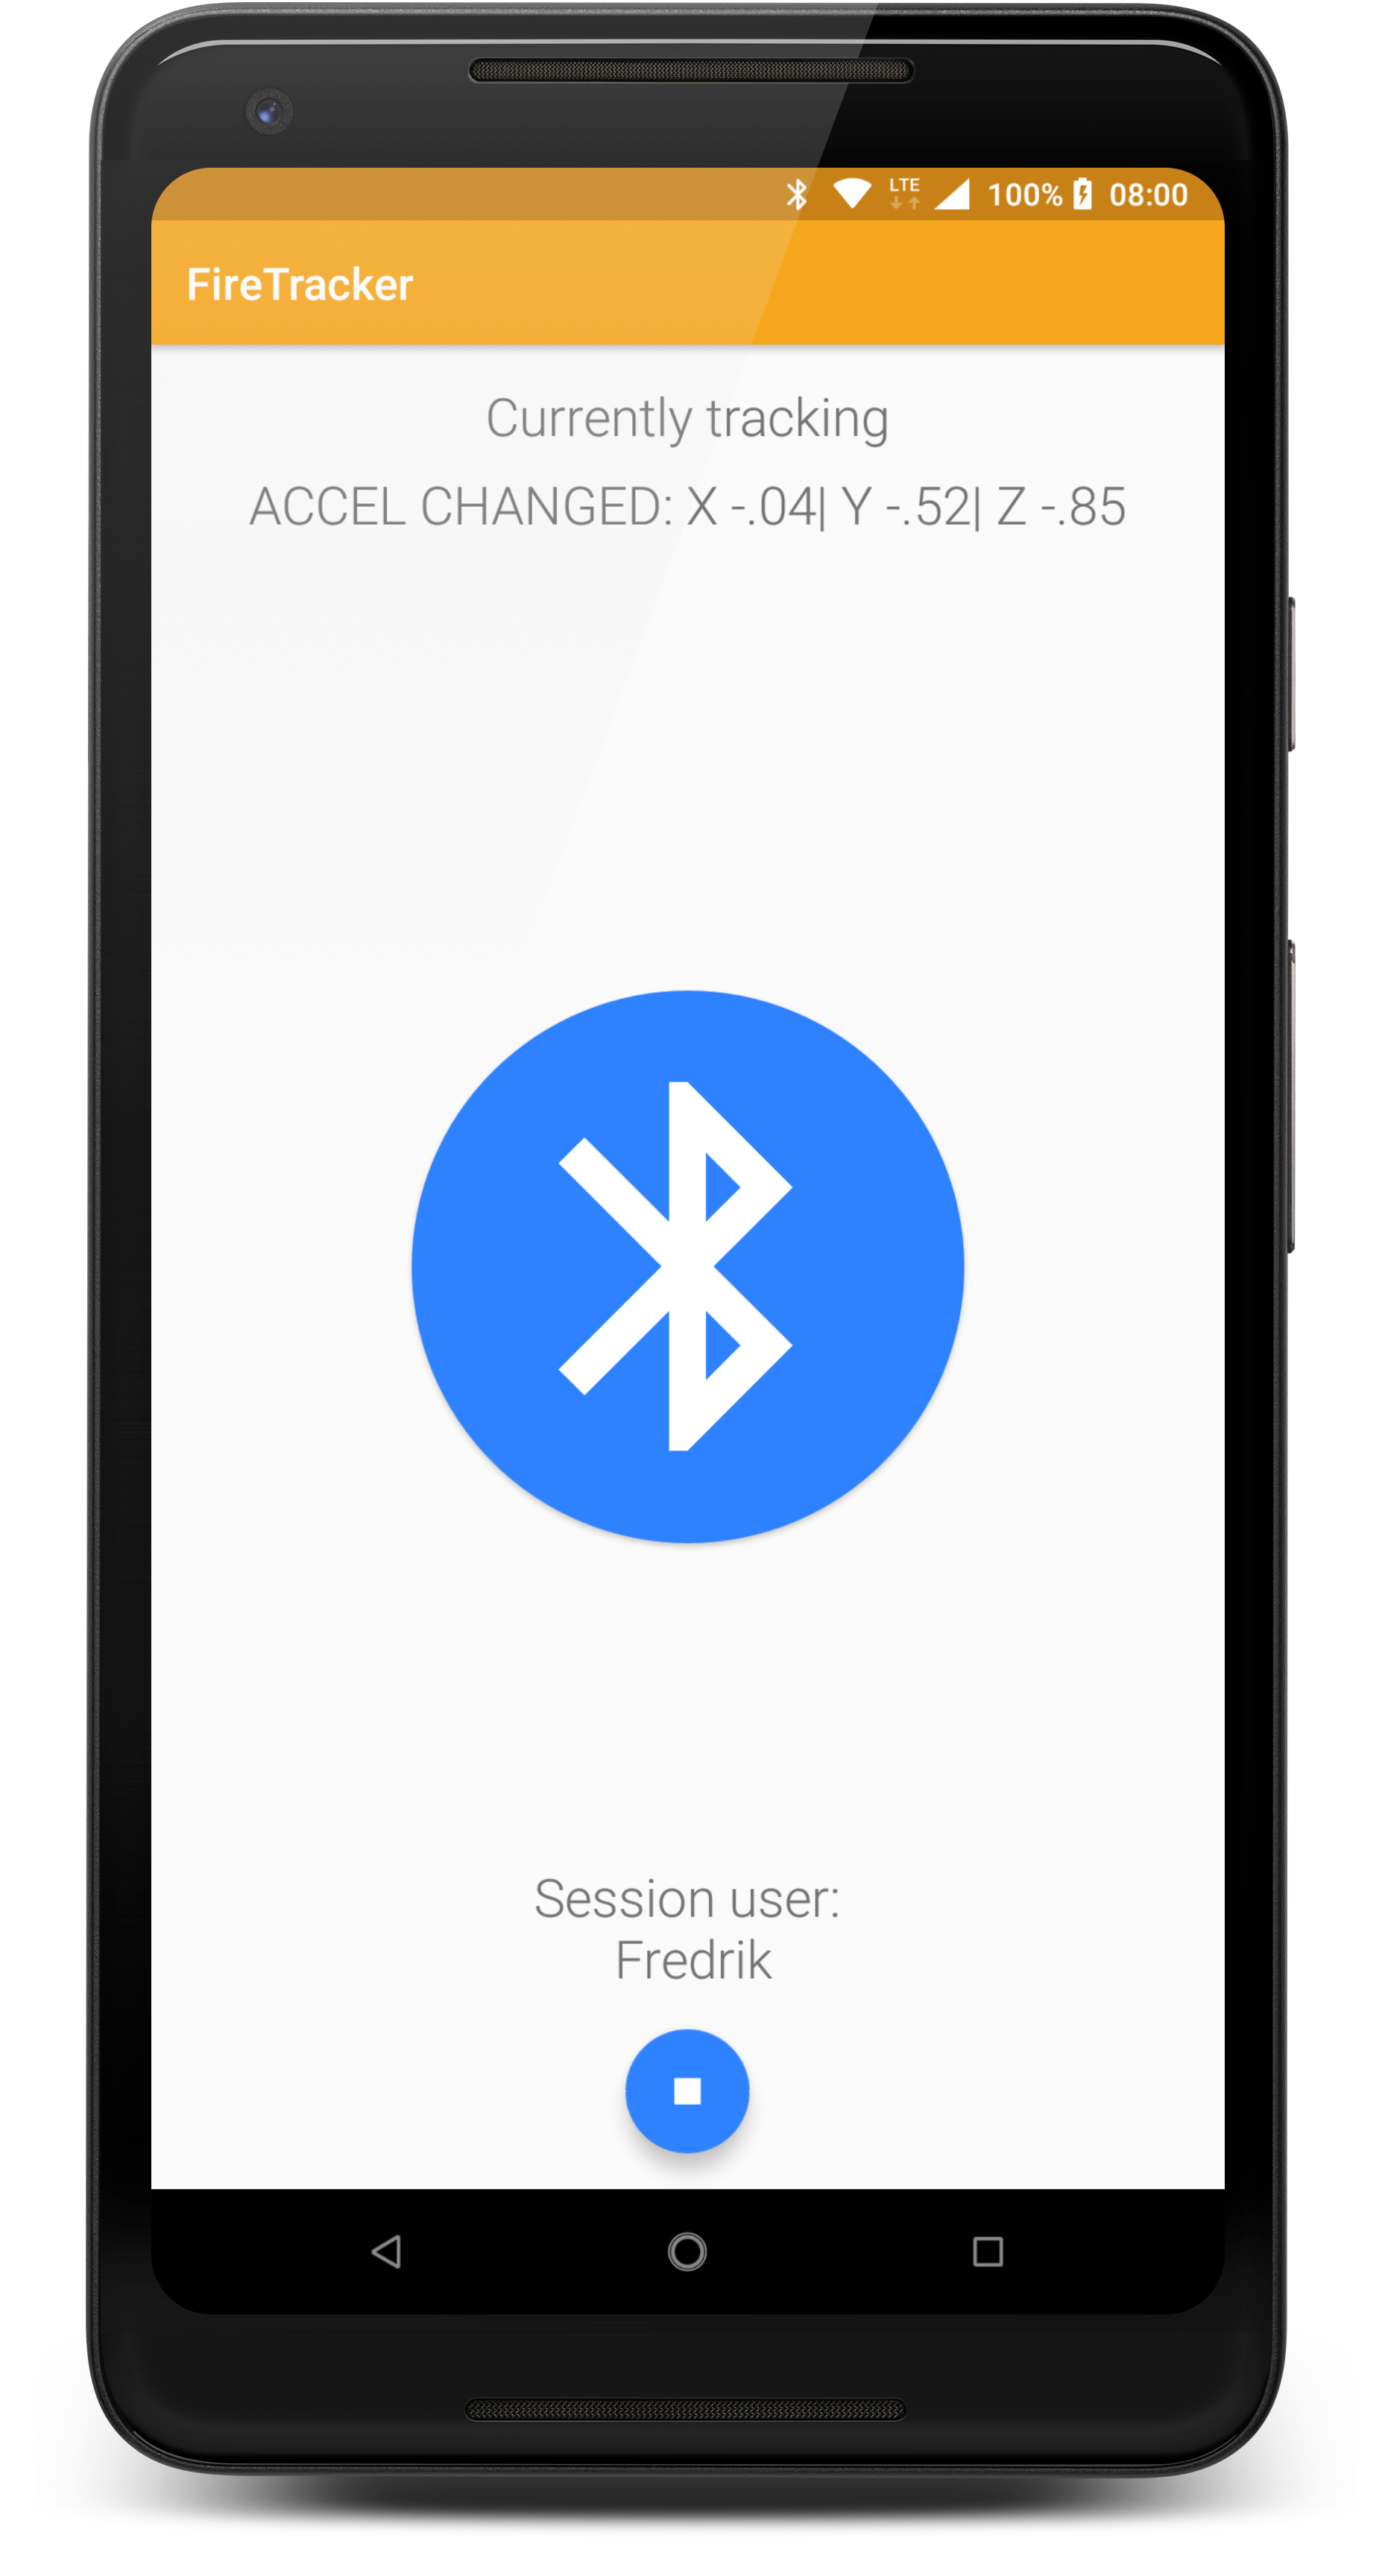
\includegraphics[width=\textwidth]{../fig/firetracker_app_old_3}
		\caption{Old design}
		\label{fig:app-old-design-tracking-iteration3}
	\end{subfigure}
	\begin{subfigure}{0.2\textwidth}
		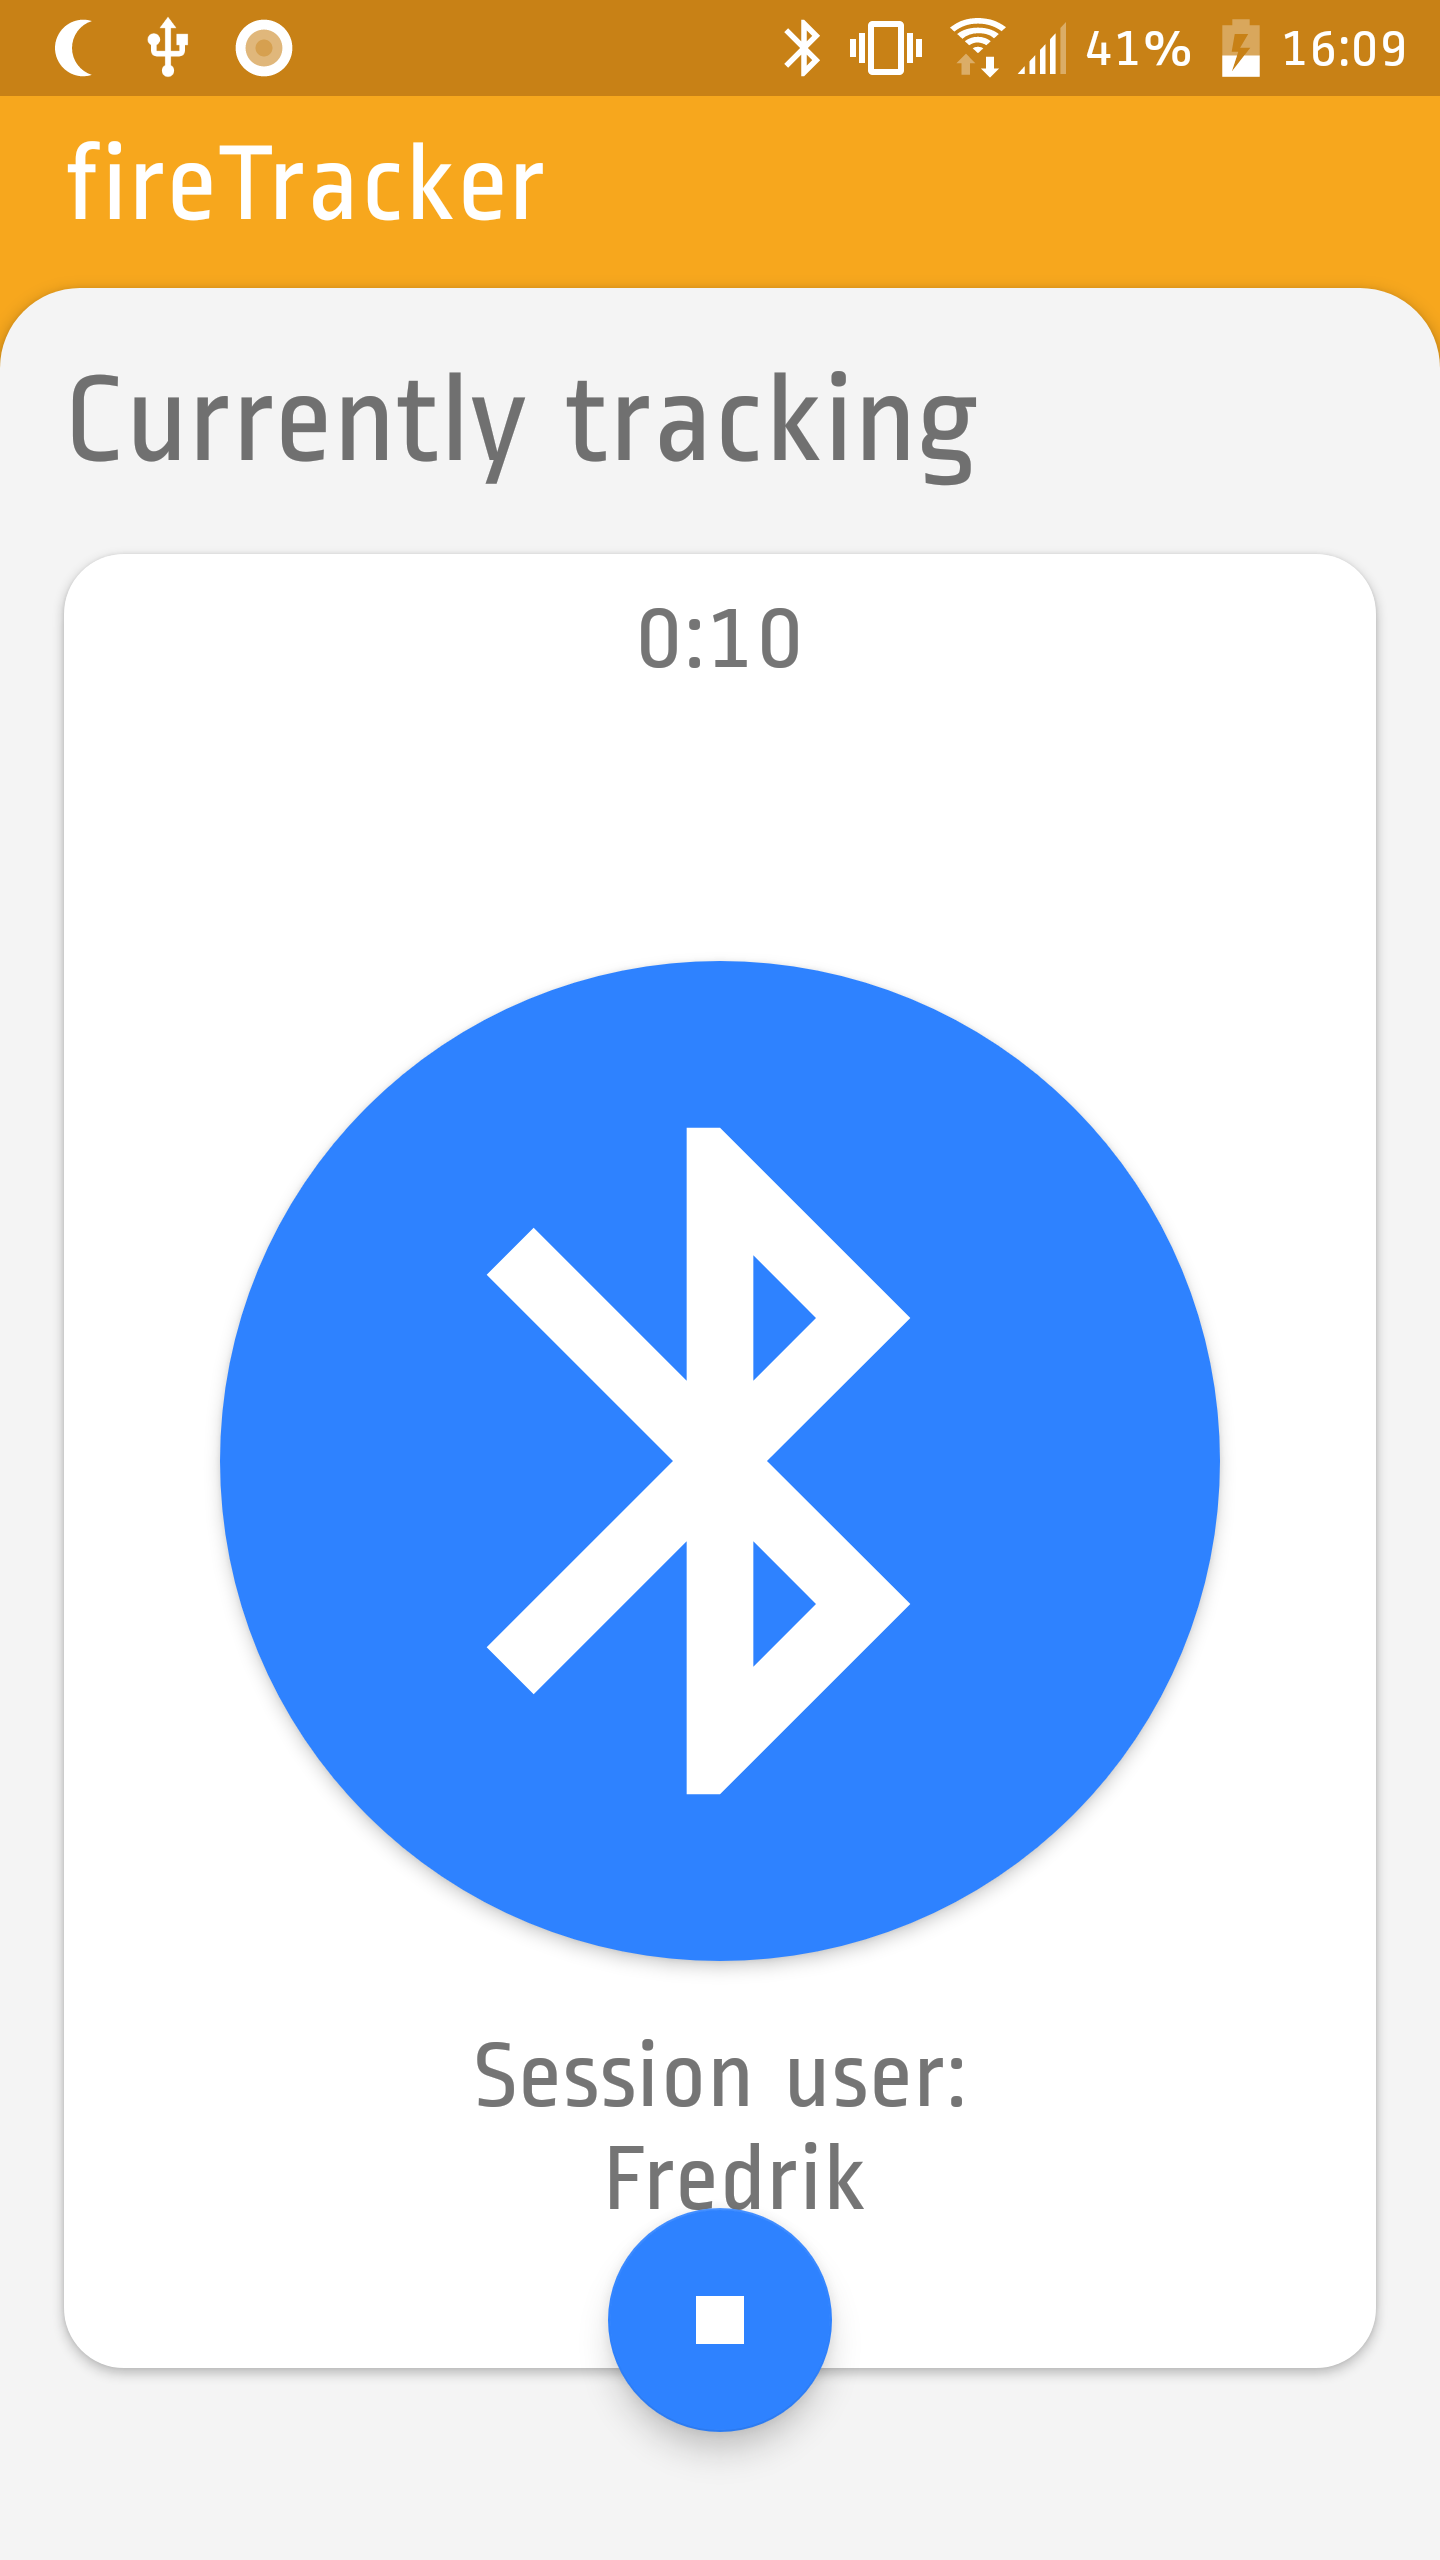
\includegraphics[width=\textwidth]{../fig/firetracker_app_new_2}
		\caption{New design}
		\label{fig:app-new-design-tracking-iteration3}
	\end{subfigure}
	\caption[Design changes in Android application]{Design changes in Android application. List of sessions screen (left) and tracking activity (right)}
	\label{fig:app-first-prototype}
\end{figure}
\todo{fix images}

As the fire department would prefer to have the system in Norwegian the app was translated into both Nynorsk and Bokmål.
The app will use the language which is set as default in the phone settings.
A safety feature was also added to prevent loss of data.
If the app is unable to upload data from a session for some reason, the user is given the opportunity to save the session locally on the device for later uploading.
This way the exercise can continue and the device can be used for another session immediately. 

On the tracking screen a timer was added to make it easier to see how long the session has lasted.
The settings for how often the phone should search for BLE signals was also changed to the shortest possible interval.

\section{Back end}
During this iteration there improvements were made to the back-end, both to the web-server part and to the data processing part.
Those changes are described in the following sections.

\subsection{Web-server}
An endpoint for deleting beacons from the database was added to the web-server during this iteration.
The other endpoints were restructured removing the ``raw''-part of the session related URLs.
Instead of specifying if the session should be unprocessed or not the default is to return processed locations if they exists, but not return all the collected data associated with a session.
This was done to reduce the amount of data that is returned, which effected the loading time of large sessions.
If one wants all the data points for a session it is possible to specify that.
When getting a list of sessions the default is to exclude both locations and data points.
All available endpoints with their description is presented in Table~\ref{tab:endpoints-2}.

\begin{table}[h]
\caption{Web-server endpoints after the third iteration}
\begin{tabular}{|p{0.2\linewidth}|p{0.15\linewidth}|p{0.15\linewidth}|p{0.4\linewidth}|}
\hline
\textbf{Relative path} & \textbf{Request Type} & \textbf{Parameters} & \textbf{Description}                                        \\ \hline
/session               & OPTIONS               &                     & Create a new session                                        \\ \hline
/sessions              & GET                   &                     & Get all sessions                                            \\ \hline
/sessions              & POST                  & Finished            & Get sessions where the finished-flag is set to ``Finished'' \\ \hline
/session:id            & GET                   &                     & Get a session with the ID ``id''                            \\ \hline
/fullsession:id        & GET                   &                     & Get a session with the ID ``id'' including datapoints       \\ \hline
/session:id            & PUT                   &                     & Update a session with the ID ``id''                         \\ \hline
/beacon                & OPTIONS               &                     & Create a new beacon                                         \\ \hline
/beacon/delete         & POST                  & Id                  & Delete the beacon with the ID ``id''                        \\ \hline
/beacons               & GET                   &                     & Get a list of all beacons                                   \\ \hline
/sessionbeacon         & POST                  &                     & Create a new beacon for a specific session                  \\ \hline
/map                   & POST                  &                     & Upload a map                                                \\ \hline
\end{tabular}
\label{tab:endpoints-2}
\end{table}

\subsection{Data processing}
\label{sec:data-processing-2}
The data processing algorithm went through a massive overhaul in this iteration.
The estimation of mid-points between two locations was removed, and the collected data were ``cleaned'' to avoid jumping back and forth between locations with short duration. 
The final version of the algorithm that was developed in this iteration is described in the following paragraphs.

The first step of the algorithm is to go through the list of datapoints and check whether each datapoint is associated with a beacon registered for this session.
If the UUID, Major and Minor value of the datapoint matches one of the beacons for the session the datapoint is kept, otherwise it is discarded.
When the list of datapoints is updated to contain only relevant data the creation of location begins.

The first datapoint in the list is chosen as the basis for the first location, using the coordinates from the beacon associated with the datapoint as the coordinates for the location.
The duration is set to zero, the start time and end time is both set to the time stamp of the datapoint, and both the walking and head movement flag is set to false.
Then for all of the remaining datapoints in the list it checks if the signal it represents is from the same beacon as the location it is currently working with.
If it is the same beacon it sets the end time of the location to the time stamp of the data point, updates the duration of the location, and checks the difference in steps and gyroscope values between the previous data point and this data point to determine if the walking and head movement flags should be set to true.

If it is a new beacon, and it has a stronger signal strength than the last received signal from the previous beacon the current location is finished and added to the list of locations.
Then a new location is created using the information from this new beacon.

When all data points are converted to locations the process of cleaning the list of locations begin.
The cleaning process compares the length of locations before and after the cleaning and is repeated until there is no change in length.
The first step of the cleaning is to go through the list of locations and check if adjacent locations have the same x- and y-coordinate.
If they are the same the two locations are merged into one.
The merged location gets the start time of the first location and the end time of the second location.
The duration of the new location is set to the sum of the two locations.
If either location has the walking set to true this flag is set to true in the new merged location, the same applies to the head movement flag.

The next step of the cleaning process is to go through the new list of locations and check if there are occurrences of two locations with the same coordinates which are separated by a location with a very short duration.
If this is the case the location in between is removed and the two other locations are merged.
Then the first step of merging adjacent locations with the same coordinates are repeated.

When the cleaning process is finished and cannot find any more locations to merge or remove the list of locations are stored in the database, and is ready to be visualized by the exercise management tool.

\section{Data specifications}
There were some minor changes to the data specifications in this iteration.
To visualize the time the smoke divers use in each location better it was decided to add the time they arrive and leave each location, in addition to the duration of the stay.
This change can be seen in Source~Code~\ref{listing:location-json-iteration3}.
All other data specifications remained as they were described in Chapter~\ref{sec:data-specifications-1}.

\begin{figure}[h]
\begin{minipage}{0.45\textwidth}
\centering
\begin{minted}
	[
	frame=lines,
	linenos
	]{json}
{
  "ID": <integer>,
  "SessionId": <integer>,
  "XCoordinate": <float>,
  "YCoordinate": <float>,
  "Duration": <integer>,
  "Walking": <boolean>,
  "HeadMovement": <boolean>
}
\end{minted}
%\captionof{listing}{Old location JSON-object}
%\label{listing:location-json-2}
\end{minipage}
\hfill
\begin{minipage}{0.45\textwidth}
\centering
\begin{minted}
	[
	frame=lines,
	linenos
	]{json}
{
  "ID": <integer>,
  "SessionId": <integer>,
  "StartTime": <integer>,
  "EndTime": <integer>,
  "XCoordinate": <float>,
  "YCoordinate": <float>,
  "Duration": <integer>,
  "Walking": <boolean>,
  "HeadMovement": <boolean>
}
\end{minted}
%\captionof{listing}{New location JSON-object}
%\label{listing:location-json-3}
\end{minipage}
\captionof{listing}{Updated Location JSON-object}
\label{listing:location-json-iteration3}
\end{figure}

\section{Testing}
\label{sec:iteration3-testing}
During this iteration some testing was done to ensure the system was ready for the final evaluation.
This testing was done on campus at the Department of Information Science and Media Studies.
A map of the floor used for the test is shown in Figure~\ref{fig:infomedia-map}.
The participants in this test was Fredrik V. Heimsæter and Edvard P. Bjørgen.

\begin{figure}[h]
	\centering
	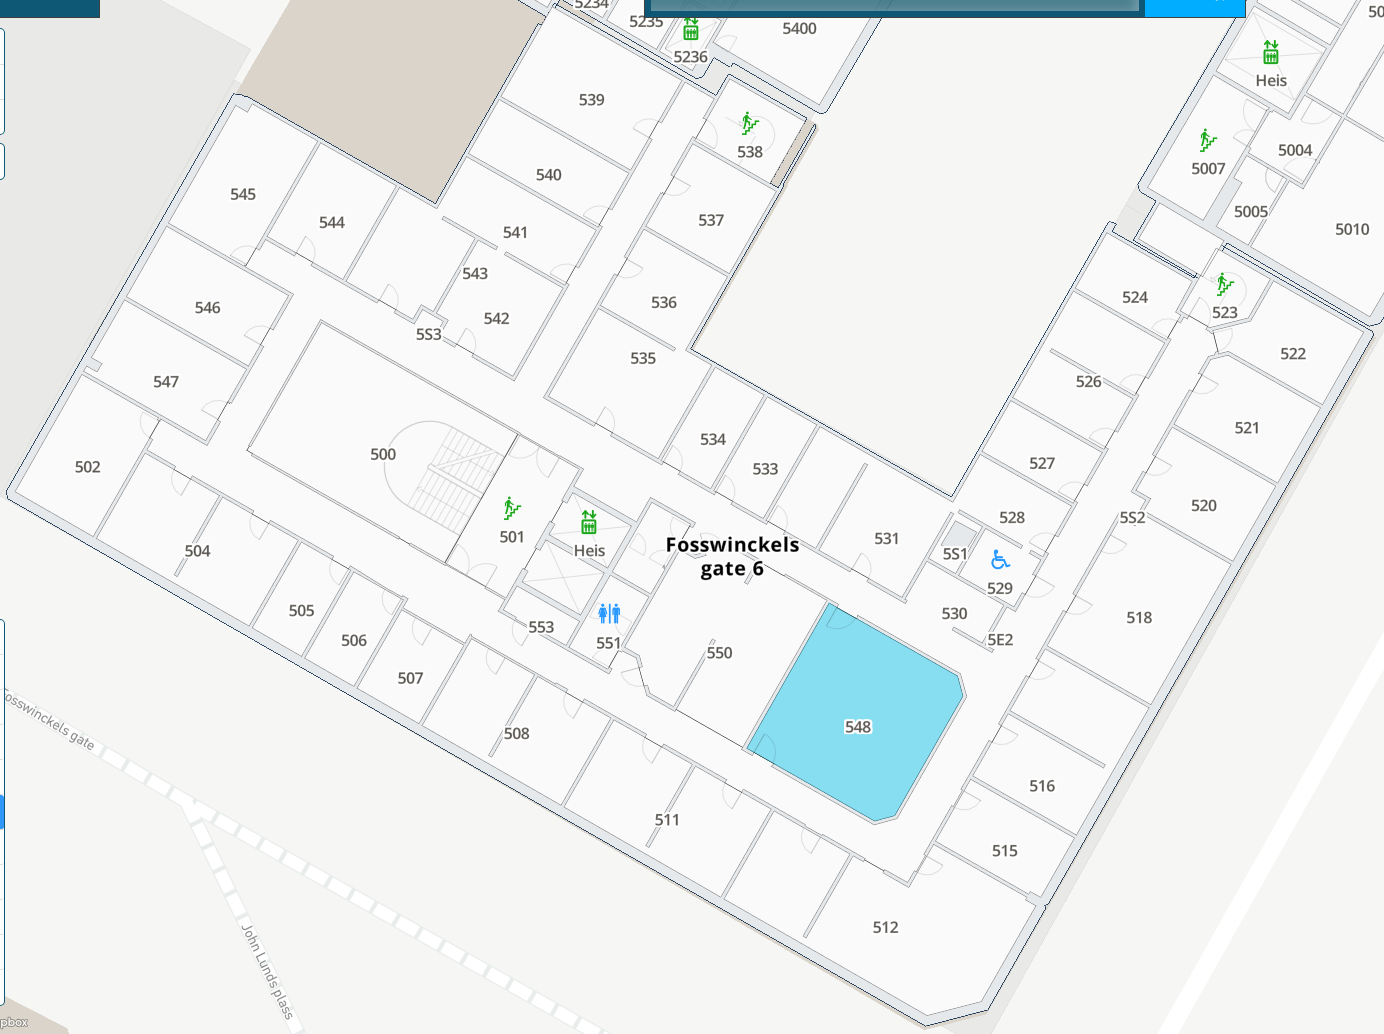
\includegraphics[width=\textwidth]{../fig/infomedia-map}
	\caption[Map of the Department of Information Science and Media Studies]{Map of the Department of Information Science and Media Studies \small(Map taken from \url{https://use.mazemap.com/})}
	\label{fig:infomedia-map}
\end{figure}

For these tests the beacons were taped to the roof along the hallways of the building.
Ideally they should have been placed inside the different rooms and offices, but that was not possible as the rooms are in use.
The floor has glass walls and some open areas between the hallways.
These tests were done with the BLE beacons from Ebeoo.
All beacons were set up with the same UUID. 
They were grouped into three different groups depending on the physical color of the beacons.
All beacons with the same color got the same Major value, and each beacon in the same group got an unique Minor value.
All beacons were set to transmit with the lowest possible signal strength.
Five different Android devices was used during the testing.

From the tests two major observations were made.
The first was that the different Android devices registered different amounts of data points when walking the same route through the building with the devices side by side.
This is probably because the manufacturers use different Bluetooth-antennas. 
The result of this observation was that the scanning interval in the Android application was set to the lowest possible value, in an attempt of forcing the devices to scan more often.
This change improved the scanning results, and the devices that previously got the least amount of data points got closer to the number of data points collected by the devices that got largest amount, but there was still a difference.
Therefore the two devices that collected the largest amount of data points was selected for the rest of the testing and the final evaluation.

The next observation was that even though the beacons were set to transmit at the lowest possible signal strength the beacons had a longer range than expected.
Because of this the devices received signals from several beacons at the same time, and the difference in RSSI between the closest beacon and a beacon 15 meters away was both small and inconsistent.
This made it hard to use any kind of measures to decide which beacon was the closest.
Another result of this was that the actual time a smoke diver spent in an area was split up into several locations with locations from other beacons with a very short duration in between.
This effect was reduced by the cleaning process described in Section~\ref{sec:data-processing-2}.

Attempts were made to reduce the signal strength of the beacons.
The beacons were partly wrapped in aluminum foil, but that did not have any significant impact on the signal strength.
The beacons were totally wrapped in aluminum foil, but that resulted in no signal received from the beacon at all.
The Android devices were wrapped in aluminum foil, and the result was that they received no BLE signals at all.

Because of time constraints a decision on how to handle this problem had to be made.
The fact that the beacons were mostly placed in the same room, or was separated by glass walls seemed like a plausible explanation of why this problem occurred.
It was also expected that spreading the beacons across different rooms with thicker walls that blocks the signals better would improve the result.
Therefore it was decided not to do anything more with the system and beacons.

\section{Summary}
This chapter described the third, and last, iteration of the development.
During this iteration the prototypes were finalized and tested.

\blankpage
\end{document}
